

\documentclass[a4paper, 12pt]{article} 
\usepackage{amsmath, amssymb, color, graphicx, enumitem}
\usepackage{fullpage} %smaller margins
\usepackage{hyperref} % hyperlinks

%font
%\usepackage[sc]{mathpazo}
%\linespread{1.05}         % Palladio needs more leading (space between lines)
%\usepackage[T1]{fontenc}

%font, libertine
\usepackage{libertine}

%word spacing
\usepackage{microtype}

%all equations get full space
\everymath{\displaystyle}

%useful shortcuts
\def\R{\ensuremath{\mathbb{R}}} %\ensuremath adds math mode, if forgotten
\def\Q{\ensuremath{\mathbb{Q}}}
\def\N{\ensuremath{\mathbb{N}}}
\def\Z{\ensuremath{\mathbb{Z}}}
\def\C{\ensuremath{\mathbb{C}}}

%shorcuts with arguments
\newcommand{\abs}[1]{\left\vert#1\right\vert} %nice absolute values
\newcommand{\bt}[1]{\textbf{#1}} %bold
\newcommand{\eq}[1]{\begin{align*}#1\end{align*}} %aligned equations
\newcommand{\cb}[1]{\centerline{\fbox{#1}}} %centered box
\newcommand{\bp}[1]{\fbox{\parbox{0.8\textwidth}{#1}}} %box paragraph
\newcommand{\norm}[1]{\left\lVert#1\right\rVert} %vector norm
\newcommand{\notimplies}{% does not imply
  \mathrel{{\ooalign{\hidewidth$\not\phantom{=}$\hidewidth\cr$\implies$}}}}
\renewcommand{\eq}[1]{\begin{align*}#1\end{align*}} %aligned equations


%colors
\definecolor{javagreen}{rgb}{0.25,0.5,0.35} %dark green color
\newcommand{\green}[1]{\textcolor{javagreen}{#1}} %command for green
\newcommand{\gray}[1]{\textcolor[gray]{0.5}{#1}} %gray text

%environment
\newcommand{\tab}{\phantom{ssss}}


\title{}
\date{}
%==tips====
%part
    %section, sub, sub
%\begin{enumerate}[resume] %continues counting
\begin{document}
\begin{center}
\section*{Training for Quiz 1}
Fundamentals of Calculus I
\end{center}

\bt{Explain and justify your thought process.}
\begin{enumerate}
    \item What's the slope of the line going through $(1, 2)$ and $(2, 10)$?\\

    \item For $f(x) = 3x + 5$, find all solutions to $3x = f(x)$. \\
    \item For $h(x) = x^2$, graph $h(x-2) + 10$. 

    \item What's the minimum value of $x^2 + 6x + 20$? \\

   For questions 5 and 6, note Apple can build an iphone 6 factory for \$100,000. Each iphone costs \$100 to produce. 
    \item Express the cost of producing iphones as a linear fuction. \\
    \item What's the total cost of producing 500 iphones? \\
\end{enumerate}

\newpage

\centerline{\bt{Solutions}}
\begin{enumerate}
    \item What's the slope of the line going through $(1, 2)$ and $(2, 10)$?\\
    \green{
    Slope answers the question: how much does y change by when $x$ increases by 1?\\
    When $x$ inceases by 1, $y$ increases from 2 to 10, implying the slope is 8.
    }

    \item For $f(x) = 3x + 5$, find all solutions to $3x = f(x)$. \\
    \green{
    No solution, as the lines are parallel.
    }
    \item For $h(x) = x^2$, graph $h(x-2) + 10$.
    \green{
    It's the graph of $x^2$ shifted to the right by 2 and up by 10:
    }

    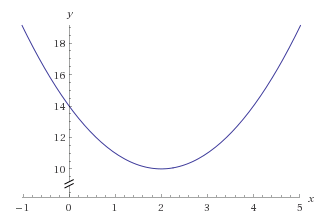
\includegraphics{graphs/x2_right_up.png}
    \item What's the minimum value of $x^2 + 6x + 20$? \\
    \green{
    The function is a parabola, facing upwards. We can relate this function to $x^2$ by completing the square:
    \eq{
    x^2 + 6x + 20 & = (x+3)^2 + \text{\underline{\hspace{0.5cm}}} \\
    & = (x+3)^2 + 11 \tag{since 9 + 11 = 20}
    }
    Therefore, the function is $x^2$ shifted left by 3 and up by 11, meaning the minimum value is 11.
    }


   For questions 5 and 6, note Apple can build an iphone 6 factory for \$100,000. Each iphone costs \$100 to produce. 
    \item Express the cost of producing iphones as a linear fuction. \\
    \green{
    There's a fixed cost of 100,000 to build the factory, then 100 per iphone. Therefore, if we let $x$ be the number of iphones we have: 
    cost = 100 x + 100,000
    }
    \item What's the total cost of producing 500 iphones? \\
    \green{
    We evaluate our function at an input of 500: 
    cost = 100*500 + 100,000 = 50,000 + 100,000 = 150,000.
    }
\end{enumerate}

\end{document}

